\documentclass[t,10pt,hyperref={
  %pdfpagemode=FullScreen,
  pdftitle = {gearshifft},
  pdfsubject = {gearshifft},
  %linktocpage=true,
  pdfborder={0 0 0},
  colorlinks=true,
  urlcolor=red,
  citecolor=red,
  linkcolor=red,
  pdfauthor={Peter Steinbach, Matthias Werner}
  }
]{beamer}
\usetheme{custom}
\def\resetbeamertemplate{\setbeamertemplate{background canvas}{ }}
\let\Tiny=\tiny
%\usepackage{lmodern}
\usepackage{tikz}
\usetikzlibrary{matrix}
\usetikzlibrary{calc}
\usetikzlibrary{positioning}
\usetikzlibrary{arrows}
\usetikzlibrary{trees}
\usetikzlibrary{backgrounds}

\usepackage[utf8]{inputenc}
\usepackage[T1]{fontenc}
\usepackage{csquotes}
\usepackage{ifthen}
\usepackage[capitalize]{cleveref} % after hyperref

\usepackage{amsmath,amstext,amsthm,array,booktabs}
\usepackage{caption}
\usepackage{xcolor}
\usepackage{graphicx}
\usepackage{subfig}
\graphicspath{{../}}
\usepackage{colortbl}
\usepackage{listings}
\usepackage{dirtree}

\usepackage[%per=slash,
%            decimalsymbol=comma,
            locale=US,
            ]{siunitx}

%%%%%%%%%%
\providecommand\thispdfpagelabel[1]{}


\lstset{literate={~} {$\sim\,$}{1}}
\lstset{upquote=true}
\lstset{language=C++,
  basicstyle=\small\fontfamily{fvm}\selectfont,%\ttfamily,
% 	columns=fullflexible,
  columns=fixed,
  keepspaces=true,
%       keywordstyle=\color{black}\bf,
%       stringstyle=\color{red}\ttfamily,
  showstringspaces=false,
  commentstyle=\color[rgb]{0.3,0.3,0.3}\textit,
%       morecomment=[l][\color{gray}]{\#},
  identifierstyle=\color{black},
  morekeywords={size_t},
  emph={__global__,__device__},
        emphstyle=\textit,
        numbers=left,
  numberstyle=\small\color{gray},
  breaklines=true,
  numbersep=5pt,
  xleftmargin=.19in,
}
% %%%%%%%%%%%%%%%%%%%%%%%%%%%%%%%%%%%%%%%%%%%%%%%%%%%%%%%%%%%%%%%%%%%%%%%%%%%%%%%

% \mode<presentation>{%
% \setbeameroption{show notes}
% }

\newcolumntype{M}{>{$\displaystyle}l<{$\vspace{1ex}}}
\title[gearshifft]{\texorpdfstring{%
    gearshifft\\[.5em]\Large The FFT Benchmark Suite\\ for Heterogeneous Platforms}}

\author[Steinbach, Werner]{\texorpdfstring{%
    \begin{minipage}[b]{.45\textwidth}
      \centering
      Peter Steinbach\\[.5em]
      {\footnotesize{Max Planck Institute of Molecular Cell Biology and Genetics\\
          01307 Dresden, Germany}}\\
      {\small{\url{steinbac@mpi-cbg.de}}}
    \end{minipage}%
    \begin{minipage}[b]{.5\textwidth}
      \centering
      Matthias Werner\\[.5em]
      {\footnotesize{Center for Information Services and High Performance Computing\\
          TU Dresden, Germany}}\\
      {\small{\url{Matthias.Werner1@tu-dresden.de}}}
    \end{minipage}}{The Author}}

\date{2017/06/20}

%%%%%%%%%%%%%%%%%%%%%%%%
\tikzset{invisible/.style={opacity=0},
      visible on/.style={alt=#1{}{invisible}},
      alt/.code args={<#1>#2#3}{%
        \alt<#1>{\pgfkeysalso{#2}}{\pgfkeysalso{#3}} % \pgfkeysalso doesn't change the path
      }
    }
\tikzset{class/.style={inner sep=5pt,font=\footnotesize}}
\newcommand{\pclass}[5][]{
\ifthenelse { \equal {#1} {} }
 {\node[class] (#5) at (#3,#4) {#2};}
 {\node[class] (#5) at (#3,#4) {%
\begin{tabular}{c}\scriptsize{<<#1>>}\\{\textbf{#2}}\end{tabular}%
};}
}
\newcommand{\pclassfill}[6][]{
\ifthenelse { \equal {#1} {} }
 {\node[class,rounded corners,fill=#6] (#5) at (#3,#4) {#2};}
 {\node[class,rounded corners,fill=#6] (#5) at (#3,#4) {%
\begin{tabular}{c}\scriptsize{<<#1>>}\\{\textbf{#2}}\end{tabular}%
};}
}

% https://tex.stackexchange.com/questions/263345/listings-and-verbatim-like-environments-in-a-tikz-node-using-newcommand
\newsavebox\mybox

\newcommand{\tkzgearshifft}{
%align=center,rounded corners,inner sep=5pt,rectangle,draw,
\begin{tikzpicture}
\tikzset{gr1/.style={}}
\tikzset{bts/.style={draw,circle,inner sep=3pt,fill=white}}
\tikzset{btc/.style={draw,circle,inner sep=3pt,fill=black}}

% fft parameters
\visible<4>{
\begin{scope}[yshift=3.75cm,xshift=-5.5cm,every node/.style={anchor=west,align=left,font=\small,draw,rectangle,rounded corners,fill=white}]

\node[fill=green!50] at (0,0) {cuFFT};
\node at (0.2,-0.4) {float, \ldots};
\node at (0.4,-0.8) {1024x1024, \ldots};
\node[fill=black,text=white] (mplc) at (0.6,-1.2) {Inplace\_Real, \ldots};

\end{scope}
}

% tree
\visible<5->{
\begin{scope}[yshift=3.5cm,xshift=-3.6cm]
\node[bts,fill=green!50] (b0) at (0,0) {};
\node[bts] (b10) at (-0.5,-0.6) {}; \draw (b10) -- (b0);
\node[bts] (b11) at (0.5,-0.6) {}; \draw (b11) -- (b0);
\node[btc] (b20) at (-0.75,-1.3) {}; \draw (b20) -- (b10);
\node[btc] (b21) at (-0.25,-1.3) {}; \draw (b21) -- (b10);
\node[btc] (b22) at ( 0.25,-1.3) {}; \draw (b22) -- (b11);
\node[btc] (b23) at ( 0.75,-1.3) {}; \draw (b23) -- (b11);
\node[font=\small] at (0, 0.4) {{\textbf{Boost}} Test Suites};
\node[font=\small] at (0,-1.7) {{\textbf{Boost}} Test Cases};

\end{scope}}

% 
\begin{scope}[xshift=1.75cm]
\begin{scope}

\visible<3->{
\pclass{{\textbf{Benchmark}}}{-2}{4}{b}
\pclass[Functor]{BenchmarkSuite}{-2}{3.2}{bs}
\pclass[Functor]{BenchmarkExecutor}{-2}{2.1}{be}
}
\pclassfill[Functor]{FFT}{-2}{1.0}{fft}{yellow}

\end{scope}
\begin{scope}

\pclassfill[Realisation]{Context}{1.5}{2.5}{ctx}{green!50}
\pclassfill[Realisation]{FFTClient}{1.5}{1.1}{impl}{green!50}
\visible<2->{
\pclass[Singleton]{Application}{1.5}{4}{app}
% \draw[rounded corners, dashed] (ctx.north west) rectangle (impl.south east);
% \draw[rounded corners] (ctx.north west) rectangle (ctx.south east);
% \draw[rounded corners] (impl.north west) rectangle (impl.south east);
\draw[rounded corners] (app.north west) rectangle (impl.south east);
}
\end{scope}
\end{scope}

\visible<-5>{
\matrix[
 minimum height=1.5em,
 matrix of nodes,
 row sep=-\pgflinewidth,
 ampersand replacement=\&,
 column sep=-\pgflinewidth,
 text depth=2.5ex,
 text height=1.5ex,
 text width=3.0em,
 align=center,
 nodes in empty cells,
 row 1/.style={nodes={fill=black!20,draw=black!50,thick,rectangle,draw,minimum width=2.5em,font=\scriptsize}}
]
(mf) at (0,-0.5) {
allocate \&
init\linebreak forward \&
|[gr1]| upload \&
|[gr1]| execute\linebreak forward \&
init\linebreak inverse \&
|[gr1]| execute\linebreak inverse \&
|[gr1]| download \&
destroy\\
};
}

\begin{scope}[thick]
\visible<-5>{
\draw (mf-1-1.north west) ++(-0.75em,0.5em) coordinate (ctl) -- ([xshift=0.75em,yshift=0.5em]mf-1-8.north east) coordinate (cr);
\draw[dotted] (ctl) -- ++(-2ex,0); \draw[dotted] (cr) -- ++(2ex,0);
\draw (mf-1-1.south west) ++(-0.75em,-0.5em) coordinate (cl) -- ([xshift=0.75em,yshift=-0.5em]mf-1-8.south east) coordinate (cr);
\draw[dotted] (cl) -- ++(-2ex,0); \draw[dotted] (cr) -- ++(2ex,0);
% total time
\draw[dashed,|-|] (mf-1-1.south west) ++(0,-1.5em) -- ([yshift=-1.5em]mf-1-8.south east) node[pos=0.5,fill=white,font=\small\itshape,align=center,anchor=north] {total time\\(measured separately)};
% (mf-1-1.south west) -- ++(0,-1.5em) -| (mf-1-8.south east) node[pos=0.25,fill=white,font=\small] {total time};
}

\visible<3->{
% \draw[-latex] (b) -- (bs);
% \draw[-latex] (fft) -- (ctl-|fft);
\draw[black!80] (b.south west) -- (b.south east);
\draw[black!80] (bs.south west) -- (bs.south east);
\draw[black!80] (be.south west) -- (be.south east);
\draw[-angle 60] (b) -- (app.west|-b);
}
\visible<4>{
  \draw[black!80, dashed] (b.south west) -- ++(-1em, 1.25em) -- ++(-5em,0); % test suite marker
  \draw[black!80, dashed] (bs.south west) -- ++(-1em,-1.5em) -- ++(-4em,0); % test suite marker
}

\visible<2->{
  \draw[-angle 60] (app) -- (ctx);
}
\draw[-angle 60] (impl) -- (ctx.south);
% \draw[densely dashed,-angle 90] (be.east) -| (impl.north);
% \draw[densely dashed,-open triangle 60] (impl) -- (fft.east|-impl) node[midway] (q) {};
\draw[-angle 90] (fft) -- (impl.west|-fft) node[midway] (q) {};
\visible<-5>{\draw[] (q.center) -- (ctl-|q);}
\end{scope}

\visible<6->{
  \node[align=left, anchor=north] (mpl) at (-1,-0.65) {Meta-Programming of loops for precision and transform, i.\,e.:\\[.5em]\usebox\mybox};
  \draw[-latex] (mpl) -- (mplc);
}
\end{tikzpicture}
}

%%%%%%%%%%%%%%%%%%%%%%%%%%%% 
\definecolor{arccl}{rgb}{0.45,0.45,0.45}
\definecolor{mc1}{rgb}{0.0, 0.0, 1.0}
\definecolor{mc2}{rgb}{0.0, 0.5, 0.5}
\definecolor{mc3}{rgb}{0.5, 0.0, 0.0}
\newcommand{\mgraymidrule}{\arrayrulecolor{arccl}\midrule\arrayrulecolor{black}}
%%%%%%%%%%%%%%%%%%%%%%%%%%%%%%%%%%%%%%%%%%%%%%%%%%%%%%%%%%%%%%%%%%%%%%%%



\newcommand{\gearshifft}{\texttt{gearshifft}}
\newcommand{\fftw}{\texttt{fftw}}
\newcommand{\cufft}{\texttt{cuFFT}}
\newcommand{\clfft}{\texttt{clFFT}}
\newcommand{\nvidia}{Nvidia}
\newcommand{\mc}[1]{\lstinline!#1!}
\newcommand{\iu}{{\mathrm{i}\mkern1mu}}

%% Todo: replace dirtree with gearshifft infos
%%        what is templated, what is runtime

\begin{document}
\frame[plain]{\titlepage}

\begin{frame}{FFTs}
  \centering
  \begin{tikzpicture}
    \begin{scope}[every node/.style={align=center, anchor=north}, xscale=1.15, yscale=2.5]
      \node[fill=yellow,inner sep=5pt,draw,rectangle,rounded corners] at (0,-0.5) {\textbf{FFTs}};
      % https://commons.wikimedia.org/wiki/File:JPEG_compression_Example.jpg
      \node at (-3, 0.0) {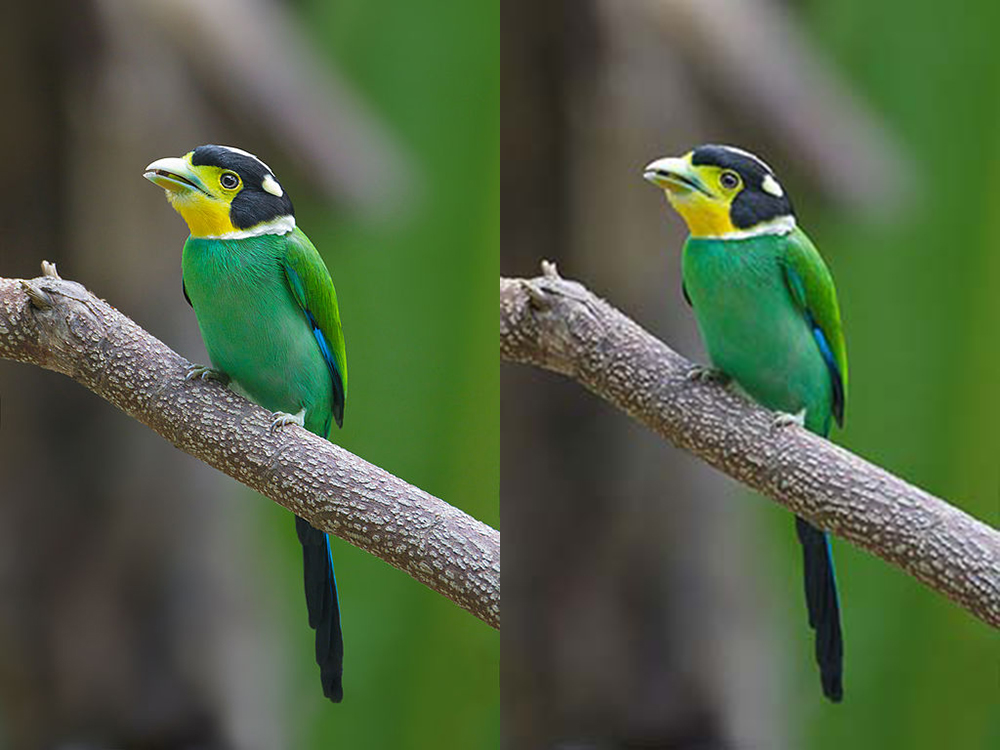
\includegraphics[width=0.25\textwidth]{jpeg-compression.jpg}\\ compression};
      % https://imagej.net/Multiview-Reconstruction
      \node at ( 3, 0.0) {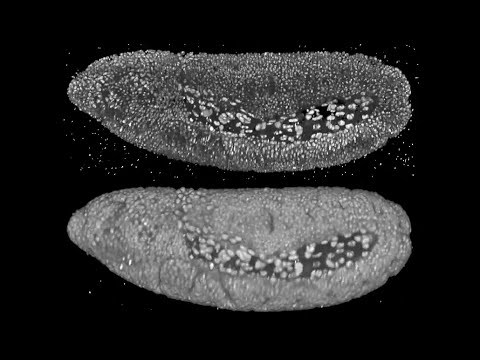
\includegraphics[width=0.25\textwidth]{imagej.jpg}\\ biology};
      % https://commons.wikimedia.org/wiki/File:Deep_learning.png
      \node at (-3, 1.0) {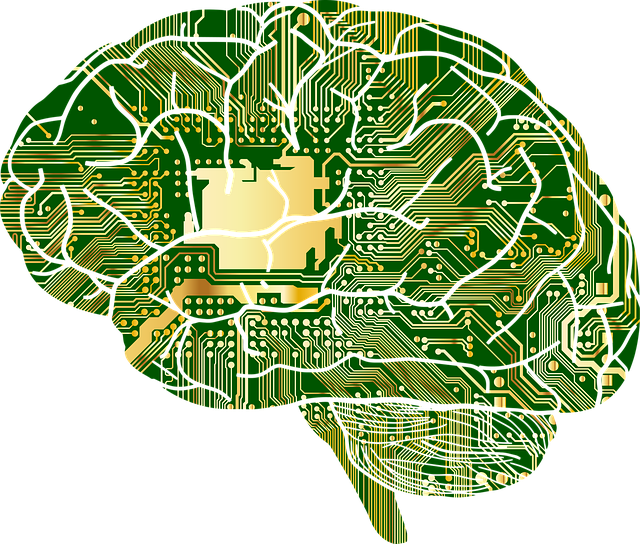
\includegraphics[width=0.21\textwidth]{deep-learning.png}\\ machine learning};
      % https://en.wikipedia.org/wiki/Trader_%28finance%29#/media/File:Philippine-stock-market-board.jpg
      \node at ( 3, 1.0) {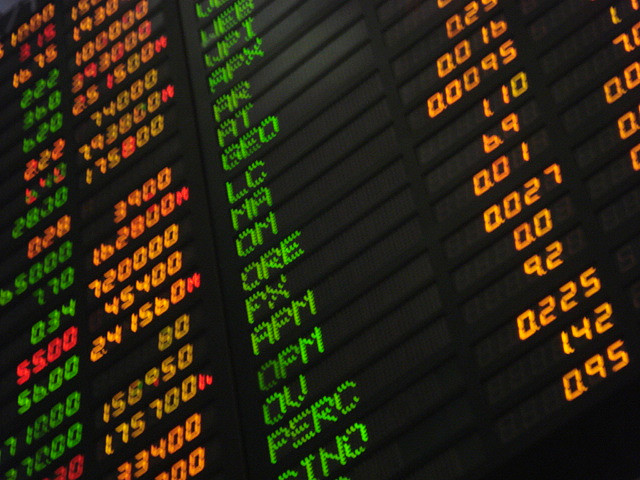
\includegraphics[width=0.25\textwidth]{Philippine-stock-market-board.jpg}\\ financial math};
      % https://de.wikipedia.org/wiki/Sinc-Funktion#/media/File:Si_sinc.svg
      \node at ( 0, 1.0) {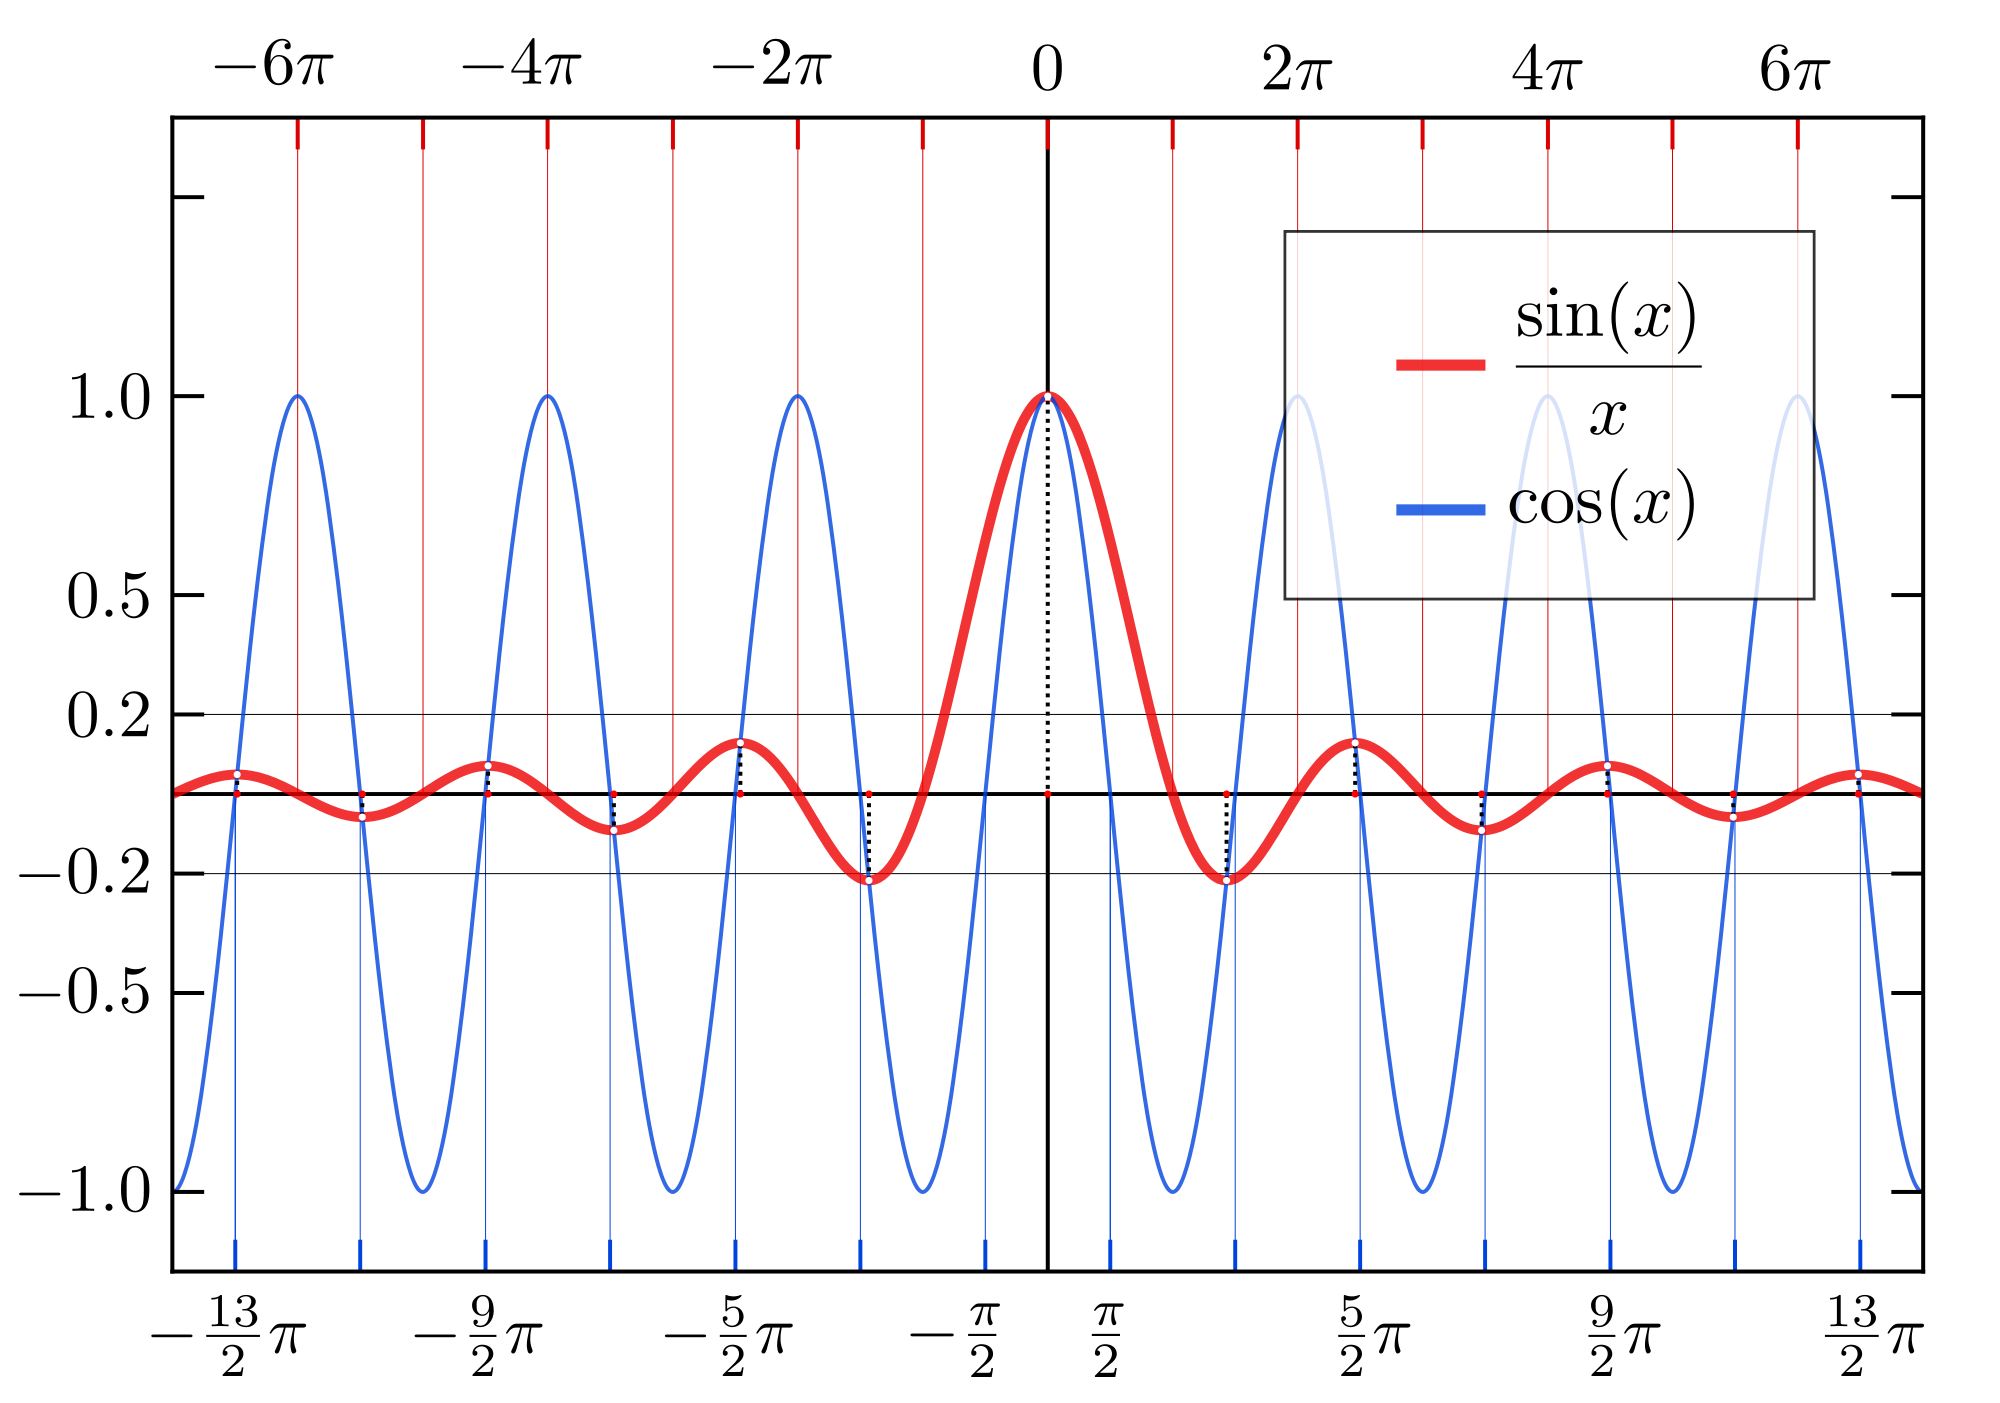
\includegraphics[width=0.25\textwidth]{sin-cos.png}\\ signal processing};
      % https://en.wikipedia.org/wiki/Interferometry#/media/File:USA.NM.VeryLargeArray.02.jpg
      \node at (-3,-1.0) {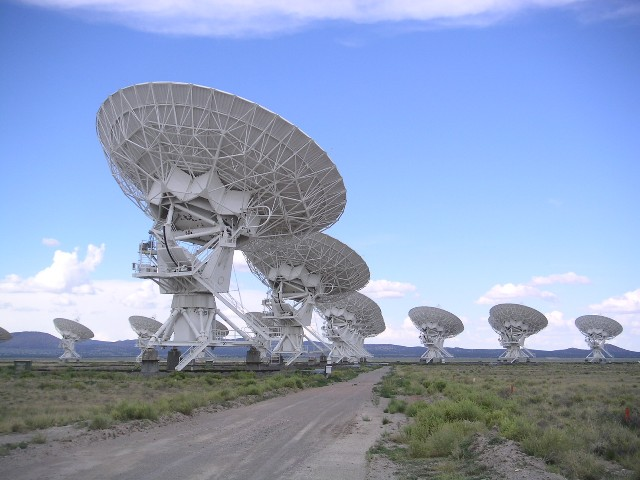
\includegraphics[width=0.25\textwidth]{usa-nm-vla.jpg}\\ astronomy};
      \node at ( 0,-1.5) {\Large\textbf{\ldots}};
      % https://en.wikipedia.org/wiki/Geology_applications_of_Fourier_transform_infrared_spectroscopy#/media/File:FTIR_spectrum.jpg
      \node at ( 3,-1.0) {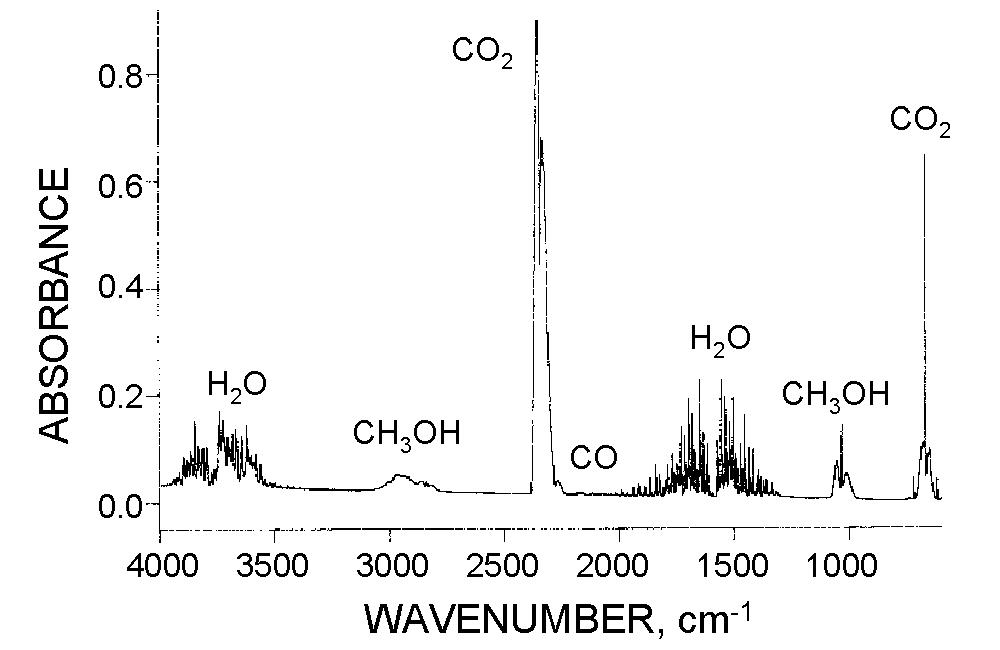
\includegraphics[width=0.25\textwidth]{FTIR_spectrum.jpg}\\ geology};
    \end{scope}
  \end{tikzpicture}
\end{frame}


\begin{frame}{Introduction}{FFTs}

  \begin{equation}
    \label{eq:dft}
    \text{DFT: }\quad X[k] = \sum_{j=0}^{n-1} x[j]\cdot\exp\left(\frac{-2\pi \iu jk}{n}\right),\quad x,X\in\mathbb{C}^n
  \end{equation}
  
  \begin{itemize}
  \item fast implementation of the discrete Fourier transform (DFT) \eqref{eq:dft}
  \item forward transform: time domain $\Rightarrow$ frequency domain
  \item factorization of $n$ and recursive decomposition smaller DFTs are computed with $\mathcal{O}(n\log n)$

    \begin{itemize}
    \item Cooley-Tukey: Radix-2 DFTs
    \item Stockham's formulations avoid incoherent memory access
    \item Bluestein's algorithm allows arbitrary and mixed radices
    \end{itemize}

  \end{itemize}

\end{frame}

\begin{frame}{FFTs}{Factor analysis}
  \centering  
  \begin{tikzpicture}
    \begin{scope}[every node/.style={align=center, anchor=north},xscale=2.5, yscale=1.75]
      \node[fill=yellow,inner sep=5pt,draw,rectangle,rounded corners] at (0,0) {\textbf{FFTs}};
    \node at (-1, 1.0) {\textbf{library}\\ cuFFT\\ clFFT\\ fftw\\ \ldots};
    \node at ( 1, 1.0) {\textbf{placeness}\\ inplace\\ outplace};
    \node at (-1, 0.0) {\textbf{precision}\\ single\\ double\\ \ldots};
    \node at ( 1, 0.0) {\textbf{transform}\\ real\\ complex};
    \node at ( 0, 1.0) {\textbf{lib-specific}\\ plan-rigor\\\ldots};
    \node at ( 0,-1.0) {\textbf{radices}\\ power-of-2\\ power-of-n\\ mixed};
    \node at (-1,-1.0) {\textbf{dim}\\ 1D\\ 2D\\ 3D\\ \ldots};
    \node at ( 1,-1.0) {\textbf{hardware}\\ CPU(s)\\ GPU\\ \ldots};
    \end{scope}
  \end{tikzpicture}

  \pause

  $\Rightarrow$ \textbf{Which FFT implementation works best on what hardware?}
  $\Rightarrow$ \textbf{What hardware is best for my domains problem configuration?}
  $\Rightarrow$ \textbf{What has changed between library versions?}
  \dots

\end{frame}


\begin{frame}[fragile]{gearshifft}

  Simplified Workflow for a single FFT benchmark of an FFT lib\\
  (e.g. 1024-FFT real-inplace single-precision):\\[.5em]
\begin{tikzpicture}[every node/.style={anchor=north west,align=left}]
    \node (a) {\textbf{FFT/lib operations}\\[.5em]
\begin{lstlisting}[numbers=none]
init_context();

init_plan();
exec_plan();
destroy_plan();

destroy_context();
\end{lstlisting}};

\node[visible on=<3->] (b) at (3.75,0) {
  \textbf{+ timer}\\[.5em]
      \begin{lstlisting}[numbers=none]
// ...

timer_start();
init_plan(...);
val = timer_stop();

// ...
  \end{lstlisting}};

\node[visible on=<4>] (c) at (7.5,0){
  \textbf{+ store times}\\[.5em]
     \begin{lstlisting}[numbers=none]
// ...

timer_start();
init_plan(...);
val = timer_stop();
store(val, PlanInit);

// ...
  \end{lstlisting}};
\end{tikzpicture}

\only<2>{
\begin{itemize}
\item data transfers not listed here
\item context has application lifetime
\item \gearshifft{} uses round-trip FFTs
\item workflow is templated by \mc{FFT.hpp}, implemented by cuFFT et. al
\end{itemize}}

\only<3>{
\begin{itemize}
\item time FFT operations
\item \gearshifft{} templates and reuses timer objects\newline
  (developer can provide own timer class)
\end{itemize}}

\only<4>{
\begin{itemize}
\item time values are collected
\item \gearshifft{} dumps results to csv in the end
\end{itemize}}

\end{frame}
  

% code used in tkzgearshifft
\begin{lrbox}{\mybox}
\begin{lstlisting}[numbers=none]
for( T_Precision : {float, double})
 for( extent : {32, 64x32, 16x16x16})
  for( T_FFT : {Inplace_Real, Outplace_Complex})
   // instantiate and run benchmark instance
\end{lstlisting}
\end{lrbox}


\begin{frame}[fragile]{gearshifft}{Basic Framework in C++/Boost}
  \centering
  \tkzgearshifft
\vspace{-2em}
\only<1>{  
  \begin{itemize}
  \item \mc{FFTClient} implements FFT workflow template class
  \end{itemize}
  }
\only<2>{  
  \begin{itemize}
  \item Application controls context object and results
  \end{itemize}
}
\only<3>{  
  \begin{itemize}
  \item Boost UTF driven generation of benchmark instances
  \end{itemize}
  }
\only<4>{  
  \begin{itemize}
  \item Boost test suites are generated by lib, precision and extents, the Boost test case is a specialized FFT client
  \end{itemize}
  }
\only<5>{  
  \begin{itemize}
  \item the benchmark tree is traversed by Boost \ldots
  \end{itemize}
  }
\end{frame}

\begin{frame}[fragile]{gearshifft}{Command-line}
%   cmake-based C++11/14 project:
% \dirtree{%
% .1 {gearshifft}.
% .2 {config}\DTcomment{config files with FFT extents}.
% .2 {inc}.
% .3 \color{mc1}{core}\DTcomment{benchmark suite header files}.
% .3 \color{mc3}{libraries}\DTcomment{FFT library instantiations}.
% .4 \color{mc3}{cufft}.
% .4 \color{mc3}{clfft}.
% .4 \color{mc3}{fftw}.
% .4 \color{mc3}{\ldots}.
% .2 {src}.
% }

% \vfill
  \begin{itemize}[<+->]
\item 
benchmark clFFT on CPU loading extents.csv dumping results to result.csv
\begin{lstlisting}[numbers=none,language=bash]
./gearshifft_clfft -f ../config/extents.csv
                   -o result.csv -d cpu
\end{lstlisting}

\item Command-line supports wildcards from Boost options
\item 
benchmark clFFT on GPU with extent=1048576, float and out-of-place real transforms
\begin{lstlisting}[numbers=none,language=bash]
./gearshifft_clfft -e 1048576
                   -r */float/*/Outplace_Real
# -r <Lib> / <Precision> / <Extents> / <Transform>
\end{lstlisting}
\end{itemize}  

\end{frame}


\begin{frame}{Results}{Validation gearshifft cufft vs. standalone cufft}
\begin{figure}[!htb]
  \centering
  \includegraphics[width=\textwidth]{figures/results_validate_cufft_legend.pdf}\\[-.5em]
  \subfloat[1024-point FFT]{\parbox[b]{0.46\textwidth}{%
    \includegraphics[width=0.5\textwidth]{figures/results_validate_cufft_a.pdf}\\
    \includegraphics[width=0.5\textwidth]{figures/results_validate_cufft_c.pdf}
    }\label{fig:tts_verify_a}}
  \hfill
  \subfloat[16777216-point FFT]{\parbox[b]{0.5\textwidth}{%
      \includegraphics[width=0.5\textwidth]{figures/results_validate_cufft_b.pdf}\\
      \includegraphics[width=0.5\textwidth]{figures/results_validate_cufft_d.pdf}
    }\label{fig:tts_verify_b}}
  \caption{\textit{gearshifft} (\cufft{}) vs. \textit{standalone} \cufft{} --  multiple timer objects \& one timer object (\textit{standalone-tts}) -- single-precision in-place real-to-complex round-trip FFTs on the K80.}
  \label{fig:verify_cufft}
\end{figure}
\end{frame}


\begin{frame}{Results}{fftw plan-rigor flags}
\begin{figure}[!htbp]
  \centering
  \includegraphics[width=\textwidth]{figures/results_plan_flags_legend.pdf}\\[-.5em]
  \subfloat[Time to Solution]{\includegraphics[width=0.49\textwidth]{figures/results_plan_flags_a.pdf}\label{fig:plan_flags_a}}
  \hfill
  \subfloat[Time for Forward Transform only]{\includegraphics[width=0.49\textwidth]{figures/results_plan_flags_b.pdf}\label{fig:plan_flags_b}}
  \caption{\fftw{} on Intel E5-2680v3 CPU with \mc{FFTW_ESTIMATE}, \mc{FFTW_MEASURE} and \mc{FFTW_WISDOM_ONLY} computing \texttt{powerof2} 3D single-precision real-to-complex in-place forward transforms.}
  \label{fig:fftw_plan_flags}
\end{figure}
\end{frame}


\begin{frame}{Results}{fftw vs. clFFT vs. cuFFT}
\begin{figure}[!tbp]
  \centering
  \includegraphics[width=\textwidth]{figures/results_non_power_of_2_legend.pdf}\\[-1em]
  \subfloat[Time for FFT]{\includegraphics[width=0.49\textwidth]{figures/results_non_power_of_2_a.pdf}\label{fig:non_power_of_2_a}}
  \hfill
  \subfloat[Time to Solution]{\includegraphics[width=0.49\textwidth]{figures/results_non_power_of_2_b_total.pdf}\label{fig:non_power_of_2_b}}
  \caption{\fftw{} and \clfft{} on Intel E5-2680v3 CPU with 24 threads versus \cufft{} on P100 GPU computing single-precision real-to-complex out-of-place forward transforms of 3D shapes.}
  \label{fig:non_power_of_2}
\end{figure}
\end{frame}


\begin{frame}{Plotting the results}{R-Shiny}
  \centering
  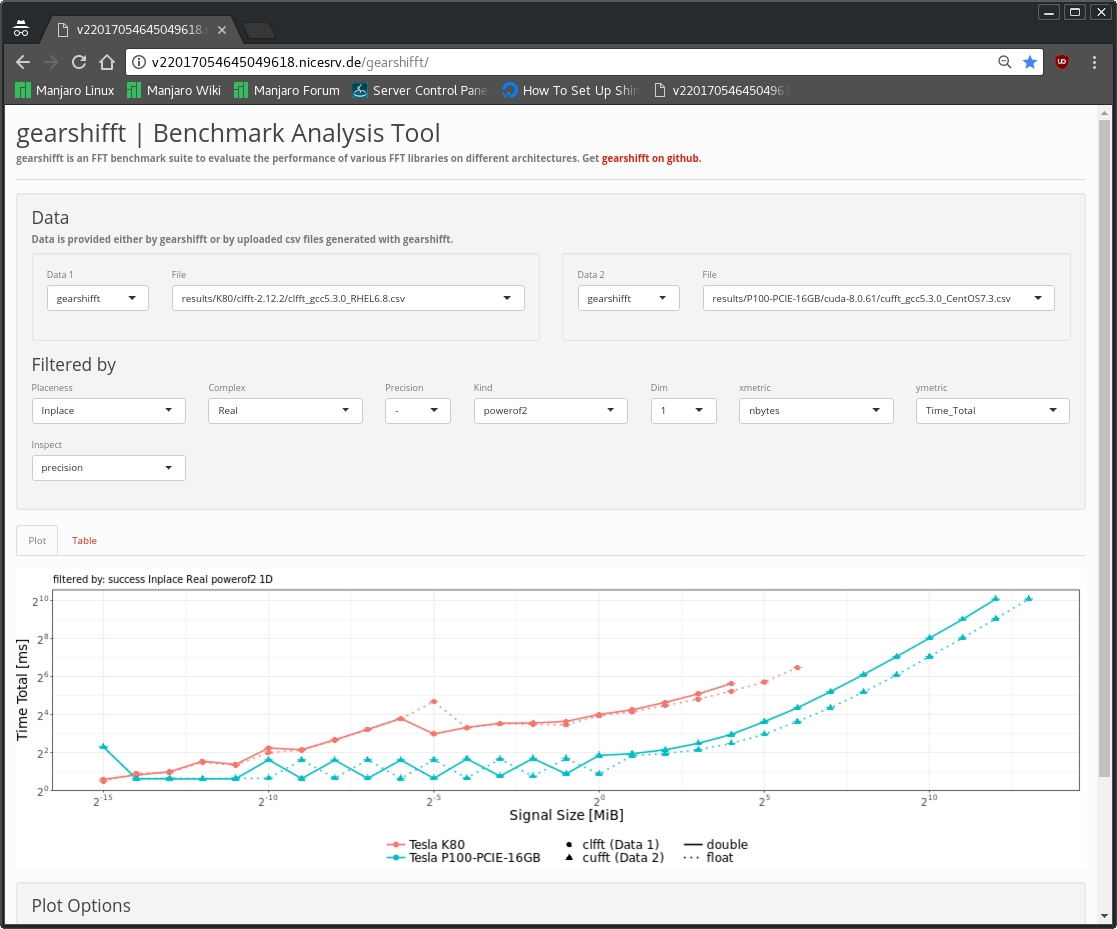
\includegraphics[width=0.8\textwidth]{rshiny.png}
\end{frame}

\begin{frame}{Summary}{}
\end{frame}


\end{document}

%%% Local Variables:
%%% mode: latex
%%% TeX-master: t
%%% End:
